% fancytikzposter.tex, version 2.1
% Original template created by Elena Botoeva [botoeva@inf.unibz.it], June 2012
% 
% This file is distributed under the Creative Commons Attribution-NonCommercial 2.0
% Generic (CC BY-NC 2.0) license
% http://creativecommons.org/licenses/by-nc/2.0/ 


\documentclass{a0poster}

\usepackage{fancytikzposter} 


%%%%% --------- Change here if you want ---------- %%%%%
%% margin for the geometry package, must be changed before using the geometry package
%% default value is 4cm
% \setmargin{4}

%% the space between the blocks
%% default value is 2cm
 \setblockspacing{1}

%% the height of the title stripe in block nodes, decrease it to save space
%% default value is 3cm
% \setblocktitleheight{3}

%% the number of columns in the poster, possible values 2,3
%% default value is 2
% \setcolumnnumber{3}

%% the space between two or more groups of authors from different institutions
%% used in \maketitle
% \setinstituteshift{10}

%% which template to use
%% N1 simple, standard look, with a colored background and gray boxes
%% N2 board with nodes
%% N3 another standard look
%% N4 envelope-like look
%% N5 with a wave-like head, original idea taken from
%%%% http://fc09.deviantart.net/fs71/f/2010/322/1/1/scientific_poster_by_nabuy-d333ria.jpg
%\usetemplate{5}

%% components of the templates
%% (the maximal possible numbers are mentioned as the parameters)
% \usecolortemplate{4}
% \usebackgroundtemplate{5}
% \usetitletemplate{3}
% \useblocknodetemplate{5}
% \useplainblocktemplate{4}
% \useinnerblocktemplate{2}


%% the height of the head drawing on top 
%% applicable to templates N3, 4 and 5
% \setheaddrawingheight{14}


%% change the basic colors
%\definecolor{myblue}{HTML}{008888} 
%\setfirstcolor{myblue}% default 116699
%\setsecondcolor{gray!80!}% default CCCCCC
%\setthirdcolor{red!80!black}% default 991111

%% change the more specific colors
% \setbackgrounddarkcolor{colorone!70!black}
% \setbackgroundlightcolor{colorone!70!}
% \settitletextcolor{textcolor}
% \settitlefillcolor{white}
% \settitledrawcolor{colortwo}
% \setblocktextcolor{textcolor}
% \setblockfillcolor{white}
% \setblocktitletextcolor{colorone}
% \setblocktitlefillcolor{colortwo} %the color of the border
% \setplainblocktextcolor{textcolor}
% \setplainblockfillcolor{colorthree!40!}
% \setplainblocktitletextcolor{textcolor}
% \setplainblocktitlefillcolor{colorthree!60!}
% \setinnerblocktextcolor{textcolor}
% \setinnerblockfillcolor{white}
% \setinnerblocktitletextcolor{white}
% \setinnerblocktitlefillcolor{colorthree}




%%% size of the document and the margins
%% A0
% \usepackage[margin=\margin cm, paperwidth=118.9cm, paperheight=84.1cm]{geometry} 
\usepackage[margin=\margin cm, paperwidth=84.1cm, paperheight=118.9cm]{geometry}
%% B1
% \usepackage[margin=\margin cm, paperwidth=70cm, paperheight=100cm]{geometry}



%% changing the fonts
\usepackage{cmbright}
%\usepackage[default]{cantarell}
%\usepackage{avant}
%\usepackage[math]{iwona}
\usepackage[math]{kurier}
\usepackage[T1]{fontenc}


%% add your packages here
%\usepackage{hyperref}  % % DISABILITATO I VIRTUAL REF


% % % DAN ADDED
\newtheorem{thm3}{Proposition}

% % % END DAN ADDED

\title{Networking-Computing resource allocation for Hard Real-Time Green Cloud applications}
%\author{Elena Botoeva\\
%  KRDB Research Centre, Free University of Bozen-Bolzano, Italy\\
%  \texttt{botoeva@inf.unibz.it}
%}
\author{ N. Cordeschi; D. Amendola; F. De Rango; E. Baccarelli\\ %\vspace{20pt}
	nicola.cordeschi@uniroma1.it; danilo.amendola@uniroma1.it; \\ derango@dimes.unical.it; enzo.baccarelli@uniroma1.it\\
	Wireless Days '14 - November 12-14, 2014 - Rio de Janeiro, Brazil }

\begin{document}

%%%%% ---------- the background picture ---------- %%%%%
%% to change it modify the macro \BackgroundPicture
\ClearShipoutPicture
\AddToShipoutPicture{\BackgroundPicture}

\noindent % to have the picture right in the center
\begin{tikzpicture}
  \initializesizeandshifts
  % \setxshift{15}
  % \setyshift{2}


  %% the title block, #1 - shift, the default value is (0,0), #2 - width, #3 - scale
  %% the alias of the title block is `title', so we can refer to its boundaries later
  \ifthenelse{\equal{\template}{1}}{ 
    \titleblock{47}{1}
  }{
    \titleblock{47}{1.5}
  }

  %% a logo can be added to the title block
  %% #1 - anchor relative to the title block, #2 - shift, #3 - width, #3 - file name
   \ifthenelse{\equal{\template}{2}}{ 
     \addlogo[south west]{(2,0)}{6cm}{unibz_b.png}
   }{
     \addlogo[south west]{(1,0.5)}{6cm}{logos/wdays14.jpg} 
     \addlogo[south west]{(41,1)}{7cm}{logos/ieee.jpg}
   }


  %% a block node, with the specified position (optional), title and the content
  %% #1 - where (optional), #2 - title, #3 - text
  %%%%%%%%%% ------------------------------------------ %%%%%%%%%%
  \blocknode{Abstract}
  {\emph{Performing real-time applications on top of virtualized cloud systems requires that the overall per-job delay due to the in-cloud processing is upper bounded in a hard way. This opens the question about the optimal dynamic joint allocation of both computing and networking resources hosted in the Cloud. This is the focus of this contribution, where we develop in \emph{closed-form} the optimal \emph{fully scalable} energy-saving scheduler for the \emph{joint} allocation of the task sizes, communication rates and processing rates in delay-constrained Clouds composed by multiple frequency-scalable parallel Virtual Machines (VMs).}
  }
  
  \blocknode%
  {Introduction and Cloud Architecture}%
  { 
  	The goal of the Green Cloud Computing is to develop models and techniques for the integrated management of computing-communication virtualized platforms, so as to provide QoS, robustness and energy efficiency. The resulting challenge is to minimize the energy usage and still meet the QoS requirements of the supported applications. About the QoS support,  an energy-saving \emph{joint} allocation of both networking and computing resources hosted in the Cloud is needed. This is the focus of this paper, where the contrasting objectives of minimizing \emph{both} networking  and computing energies in \emph{real-time} applications running on top of virtualized Clouds are cast in the form of a suitable \emph{constrained} optimization problem.
	\begin{tikzfigure}[The Considered NetDC architcture.]
	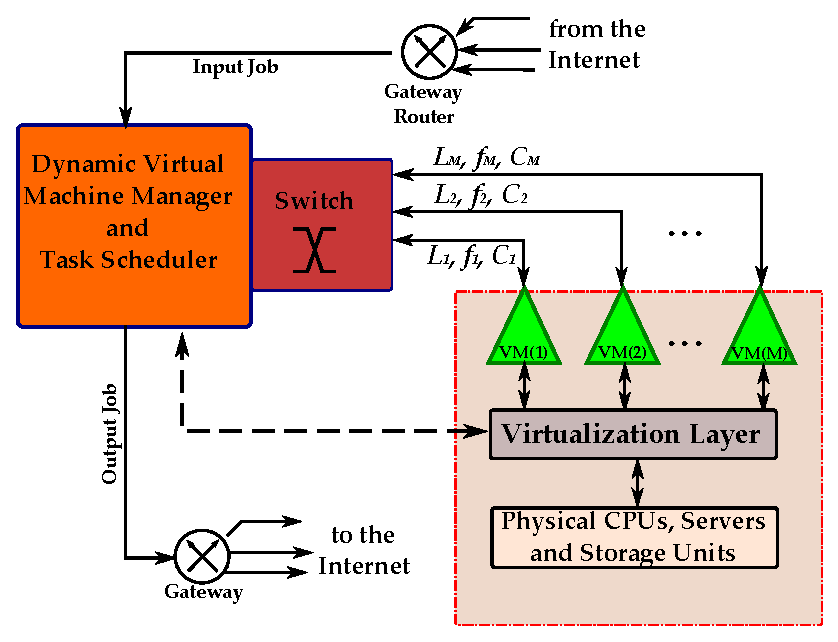
\includegraphics[width=0.6\columnwidth]{images/Modello.eps}
	\label{fig:0}
	\end{tikzfigure}
  }

  %% by default, the position of the new block node is right below the previous
  %% block node, stored in (currenty)
  %% box is the alias of the previous block, so we can refer to its boundaries

  %%%%%%%%%% ------------------------------------------ %%%%%%%%%%
  \blocknode{Problem setup and optimal resource allocation}%
  {
  	Task sizes: $\{L_i,\,i=1,\ldots,M\}$ communication rates $\{C_i,\,i=1,\ldots,M\}$ and computing rates $\{f_i,\,i=1,\ldots,M\}$, of the DVFS-enabled VMs,
  	so as to minimize the overall computing-plus-networking energy:
  	\begin{equation}\label{eq:energy-tot}
  	\mathcal{E}_{tot}\triangleq\sum_{i=1}^M\mathcal{E}_c(i)+\sum_{i=1}^M\mathcal{E}^{net}(i)\;\;(Joule),
  	\end{equation}
  	
  	On the worst case of sequential activation, the corresponding delay-constraint becomes:
  	\begin{equation}\label{eq:sequential-delay}
  	\small
  	\left[\sum_{i=1}^M2D(i)\right]+\max_{i=1,\ldots,M}\{\Delta(i)\}\leq T_t.
  	\end{equation}
  	Posing  $\Delta_{max}\triangleq\max_{i=1,\ldots,M}\{\Delta(i)\} (sec)$, the constrained optimization problem (COP): 
  	
  	\begingroup
  	\allowdisplaybreaks
  	\begin{subequations}\label{eq:probl}
  	\small
  	\renewcommand{\theequation}{\theparentequation.\arabic{equation}}
  	\begin{align}
  	&\label{eq:obiettivo}\hspace{-0.4cm}\min_{\{C_i,f_i,L_i\}}\sum_{i=1}^{M}\Psi_i\left(\frac{f_i}{f_i^{\max}}\right)
  	\mathcal{E}_i^{\max}+k_e\left(f_i-f_i^0\right)^2+2P_i^{net}\left(\frac{L_i}{C_i}\right)\\
  	&\label{eq:constr-Deltai}\mbox{s.t.:    } \left(L_i\right)/f_i\leq\Delta(i),\;\; i=1,\ldots,M,\\
  	&\label{eq:constr-Ltot}\sum_{i=1}^{M}L_i= L_{t},\;\;\;\;\;\;\;\;\;\;\;\;\;\;\;\;\;\;\sum_{i=1}^{M}2D(i)+\Delta_{max}\leq T_t,\\
  	%&\label{eq:constr-Tserv}\sum_{i=1}^{M}2D(i)+\Delta_{max}\leq T_t,\\
  	%&\label{eq:constr-Ctot}\sum_{i=1}^M C_i\leq C_{tot},\\
  	&\label{eq:constr-fi}\hspace{-0.3cm}0\leq f_i\leq f_i^{max}; L_i\geq 0; 0\leq C_i\leq C_{max},\;i=1,\ldots,M.
  	\end{align}
  	\end{subequations}
  	\endgroup
  	$f_i$  is the variable to be optimized, while  $f_i^0$  describes  the  "current" state of the VM$(i)$
  }
  
  \vspace{3cm}
  \blocknode{Authors}
  {
  	
  	\begin{minipage}[t]{0.23 \linewidth}
  	\centering
  	Nicola Cordeschi\\
  	Sapienza University of Rome
  	\begin{tikzfigure}[]
  	
\includegraphics[height=7cm]{authors/nicola_cordeschi.eps} %width=0.7\columnwidth
  	\end{tikzfigure}
  	\end{minipage}
  	%
  	\begin{minipage}[t]{0.23 \linewidth}
 	\centering
  	Danilo Amendola\\
  	Sapienza University of Rome
  	\begin{tikzfigure}[]
  	
\includegraphics[height=7cm]{authors/danilo_amendola.eps}
  	\end{tikzfigure}
  	\end{minipage}
  	%
  	\begin{minipage}[t]{0.23 \linewidth}
	\centering
  	Floriano De Rango\\
  	University of Calabria
  	\begin{tikzfigure}[]
  	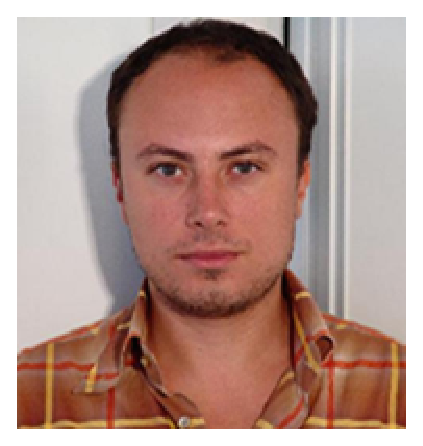
\includegraphics[height=7cm]{authors/floriano_derango.eps}
  	\end{tikzfigure}
  	\end{minipage}
  	%
  	\begin{minipage}[t]{0.23 \linewidth}
  	\centering
  	Enzo Baccarelli\\
  	Sapienza University of Rome
  	\begin{tikzfigure}[]
  	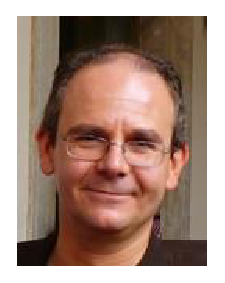
\includegraphics[height=7cm]{authors/enzo_baccarelli.eps}
  	\end{tikzfigure}
  	\end{minipage}
   }
 	
	\startsecondcolumn

  %%%%%%%%%% ------------------------------------------ %%%%%%%%%%
  %\blocknodew[($(currenty)-(3.5,0)$)]{30}{Variable Width Block Nodes} %
  \blocknode %
  {Effects of the networking powers and Hibernation} %
  {
  	To evaluate the effect on  $\mathcal{E}_{tot}^*$  of the networking powers, we have set: $T_t=500$ $(ms)$, $C_{max}=150$ $(Mbit/s)$,
  	$L_t=10$ $(Mbit)$, $k_e=0.05 (mJ)/(MHz)^2$, $f_i^{max}=100$ $(Mbit/s)$, $f_i^{0}=0$ $(Mbit/s)$, $\mathcal{E}_i^{max}=1$ $(mJ)$, $\Delta(i)=1$ $(s)$.
  	We have evaluated $\mathcal{E}_{tot}^*$  (\emph{Joule}) for the following three network scenarios: \emph{i)} $P_i^{net}=0$ $(mW)$ (i.e., no communication costs); \emph{ii)} $P_i^{net}=1$ $(mW)$ (i.e., homogeneous communication costs); and, \emph{iii)} $P_i^{net}=1+0.25(i-1)$ $(mW)$, for $i=1,\ldots,M$ (i.e., heterogeneous communication costs).
  	
  	\vspace{-30pt}
  		\begin{minipage}[t]{0.5 \linewidth}
  		\flushleft
  		\begin{tikzfigure}[Effects of the networking power demands on the Cloud performance.]
  		\includegraphics[width=1\columnwidth]{images/Costo-Totale-al-Variare-Potenza-width2.eps}\label{fig:1}
  		\end{tikzfigure}
  		\end{minipage}
  		\begin{minipage}[t]{0.5 \linewidth}
  		\begin{tikzfigure}[Optimal processing rates and optimal workloads for the application scenario of Numerical Results.]
  		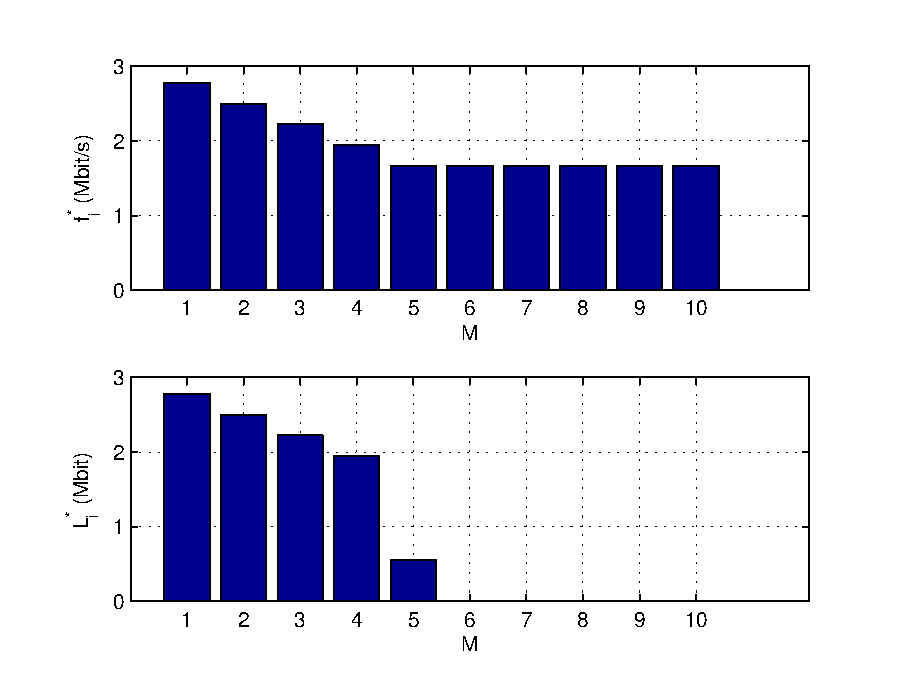
\includegraphics[width=0.8\columnwidth]{images/Bar-fopt-Lopt.eps}\label{fig:2}
  		\end{tikzfigure}
  		\end{minipage}
	}

    
  %%%%%%%%%% ------------------------------------------ %%%%%%%%%%
  \blocknode%
  {Feasibility issues and optimal scheduling}%
  {
  	%\begin{thm3}\label{prop:feas}
  	\vspace{-30pt}
  		\begin{minipage}[]{0.3\linewidth}
  		\flushleft
		The following inequality:\\
		\vspace{1pt}$\:$
  		\end{minipage}
  		\begin{minipage}[b]{0.70 \linewidth}
		\begin{align}\label{eq:feas}
		\small L_t\leq\min\left\{\sum_{i=1}^{M}f_i^{\max}\Delta(i);\frac{C_{max}}{2}\left(T_t-\Delta_{max}\right)\right\},
		\end{align}
  		\end{minipage}
  		%
%  	\begin{align}\label{eq:feas}
%  	\small
%  	&\textbf{The following inequality:}& L_t\leq\min\left\{\sum_{i=1}^{M}f_i^{\max}\Delta(i);\frac{C_{max}}{2}\left(T_t-\Delta_{max}\right)\right\},&
%  	\end{align}
  	is necessary and sufficient condition for the feasibility of the constrained optimization problem
  	in \textit{COP}.
  	%\end{thm3}

	
	%\begin{thm3}\label{prop:opt-scheduler}
	Let the constrained optimization problem in \textit{COP} be feasible. Thus, its solution equates (Case of quadratic energy consumption function).
	
	As already pointed, the form assumed by $\Phi(\eta)$ for DVFS-based CMOS CPUs is generally well approximate by quadratic one. In this case, for the optimum rate we have the following simple expression:
	
	\begin{minipage}[b]{0.55 \linewidth}
		\flushleft
		\begin{align}\label{eq:fopt-quad}	f_i^*=\left[\gamma_if_i^0+\delta_i[\mu^*-2P_i^{net}/C_{max}]_+\right]_{f_i^{min}}^{f_i^{max}},
		\end{align}
	\end{minipage}
	\begin{minipage}[b]{0.40 \linewidth}
		\begin{subequations}\label{eq:controllers}
		\small
		\renewcommand{\theequation}{\theparentequation.\arabic{equation}}
		\begin{align}
		% &\label{eq:fopt}f_i^*=\left[\pi_i^{-1}\left(2k_ef_i^0+[\mu^*-2P_i^{net}/C_{max}]_+\Delta(i)\right)\right]_{0}^{f_i^{max}}\\
		&\label{eq:Lopt}L_i^*=\bold{1}_{[\mu^*>2P_i^{net}/C_{max}]}\left(f_i^*\Delta(i)\right),\\
		&\label{eq:Copt}C_i^*=C_{max}\bold{1}_{[L_i^*>0]}.
		\end{align}
		\end{subequations}
	\end{minipage}
	

	where $\gamma_i$ and $\delta_i$ are given by:
	\begin{equation}
	\label{eq:soglia_1}\gamma_i\triangleq\frac{2k_e}{2k_e+2\mathcal{E}_i^{max}/(f_i^{max})^2},\;\; \delta_i\triangleq\frac{\Delta(i)}{2k_e+2\mathcal{E}_i^{max}/(f_i^{max})^2}.
	\end{equation}

	%\footnote{$[x]_a^b$ indicates $\min\{\max\{x;a\};b\}$, while  $\textbf{1}_{[A]}$ is the (binary-valued) indicator function of the  $A$  event.}:
	
	The scalar $\mu^*\in\mathbb{R}_0^+$ in $f_i^*$ plays the role of a Lagrange multiplier and it is computable as the solution of the following algebraic equation:
	$
	\sum_{i=1}^ML_i(\mu)=L_t.
	$
	%\end{thm3}
    % 
    The optimal scheduler hibernates VM$(i)$ when the following \emph{hibernation condition} is met (see Fig. \ref{fig:2}):
     \begin{equation}\label{eq:hib-cond}
     \mu^*<2P_i^{net}/C_{max},\,i=1,\ldots,M.
     \end{equation}
  }

  
  %%%%%%%%%% ------------------------------------------ %%%%%%%%%%
  \blocknode{Average energy consuption under random workload}%
  {
%  	For the heterogeneous network scenario already considered in Fig.\ref{fig:3} reports the \emph{average} energy consumptions of the optimal scheduler when the submitted workload is \emph{randomly} time-varying, that is, when the size $L_t$ of the job submitted at the beginning of each $T_t$-long round time is the outcome of a random variable (r.v.) evenly distributed over the interval $6$ - $10$ $(Mbit)$. Specifically, at the first round of the carried out simulations, all the source frequencies  $f_i^0$  in \eqref{eq:obiettivo} are reset. Afterwards, at the  $k$-th round, each $f_i^0$ is set to the corresponding optimal value $f_i^*$  already computed at the previous  $(k-1)$-th round.
  	%For each $M$, each operative setting runs on $50000$ rounds and, then, all the reported numerical data are averaged or more than $100$ instances, so as to guarantee that each simulated point retains $95\%$ confidence interval with at least a $10\%$ precision degree.
The plots of Fig.\ref{fig:3} may be considered representative of application scenarios where the energy due to frequency switching energy overhead is low (e.g., $k_e=0.005$ $Joule/(MHz)^2$), medium (e.g., $k_e=0.05$ $Joule/(MHz)^2$) and high (e.g., $k_e=0.5$ $Joule/(MHz)^2$). Interestingly, these plots show that: \emph{i)} the average energy consumption (quickly) increases for increasing $k_e$'s; and, \emph{ii)} the optimal number $M^*$ of VMs to be instantiated decreases for growing $k_e$'s.

%Furthermore, it is worthwhile to note that the average energy consumptions of Fig.\ref{fig:3} are of about $50\%$ less than the corresponding ones previously reported in Fig.\ref{fig:2} for the case of time-invariant deterministic job sizes $L_t$'s. This is, indeed, a further consequence of the hibernation phenomena. 
The plots of Fig.\ref{fig:4} reports the optimal allocations of the processing rates at the $1$\emph{th} round (red bars) and at the $10$\emph{th} round (blue bars) for the aforementioned heterogeneous networking case of Fig.\ref{fig:2}. The trend emerging from the plots of Fig.\ref{fig:4} is that, round-by-round, some of VMs tend to be consolidated and permanently loaded, while the remaining ones gracefully pass from the hibernation state to the off one.

	\vspace{-35pt}
	\begin{minipage}[t]{0.5 \linewidth}
	%\flushleft
	\begin{tikzfigure}[Average energy consumption of the optimal scheduler in the presence of randomly time-varying workload.]
	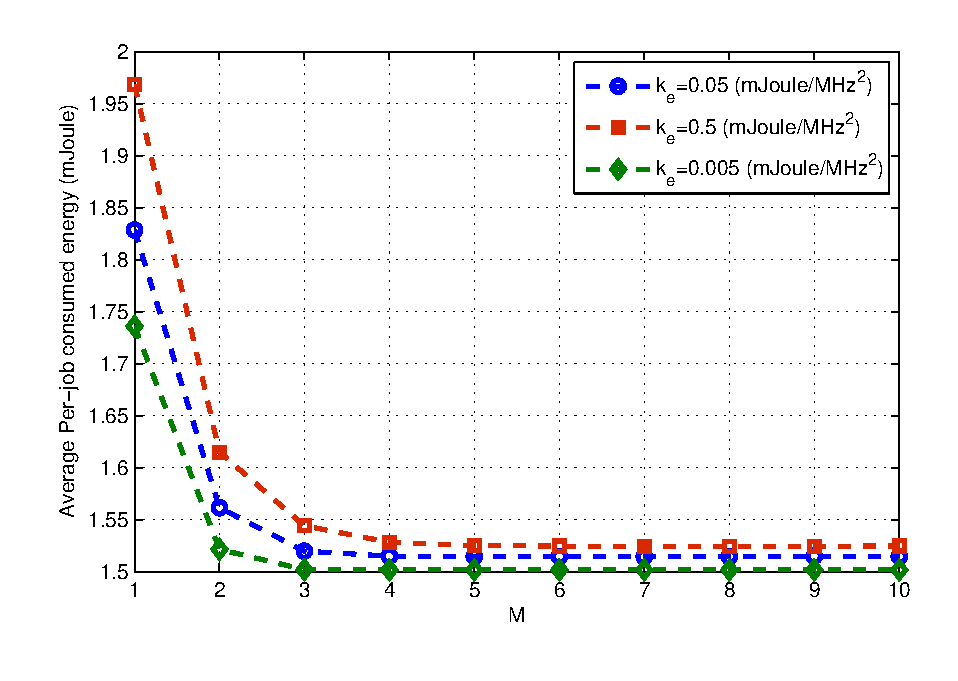
\includegraphics[height=11.5cm]{images/Cost-Tot-L-random-width2.eps}
	\vspace{-20pt}
	\label{fig:3}
	\end{tikzfigure}
	\end{minipage}
	\begin{minipage}[t]{0.45 \linewidth}
	\begin{tikzfigure}[Allocation of the processing rates at the $1$\emph{th} round (red bars) and $10$\emph{th} round (blue bars).]
	\includegraphics[height=11.5cm]{images/One-Ten-Rounds}
	\vspace{-20pt}
	\label{fig:4}
	\end{tikzfigure}
	\end{minipage}
      
%    \begin{tabular}[t]{ll}
%      \begin{minipage}{0.5\linewidth}
%        \innerblock{Theorem} {Statement}
%      \end{minipage}
%      & 
%      \textbackslash innerblock\{Theorem\}\{Statement\}\\
%
%      \begin{minipage}{0.5\linewidth}
%        \innerblockplain[colorone!80!]{Text}
%      \end{minipage}
%      &
%      \textbackslash innerblockplain[colorone!80!]\{Text\}\\ 
%
%      \begin{minipage}{0.5\linewidth}
%        \coloredbox{colorthree!50!}{Text}
%      \end{minipage}
%      &
%      \textbackslash coloredbox\{colorthree!50!\}\{Text\}
%    \end{tabular}
%
%    \vspace{0.5cm}
%    The default figure environment does not work within a tikzpicture. I created
%    a new figure environment that can be used instead, based on the code sent by
%    Stephan Thober.
%    \begin{itemize}
%    \item[] \textbackslash begin\{tikzfigure\}[Caption]\\
%      \ldots\\
%      \textbackslash end\{tikzfigure\}
%    \end{itemize} 
%    % 
%
%	\emph{note}
  }


  %% to place the next node centered vertically in the second column, we can
  %% obtain the y-coordinate of the previous node using macro
  %% \getcurrentrow{note}, where note is the alias of the callout node, and
  %% then specify the coordinate of the next node using coordinate (currentrow)
  %\getcurrentrow{note}
	%\getcurrentrow{note}
	
  %% a plain block
  %% #1 - rotate angle (optional), #2 - where, #3 - width, #4 - title, #5 - text
  %%%%%%%%%% ------------------------------------------ %%%%%%%%%%
  \plainblock{($(currenty)$)} %-(xshift) + (xshift) -(yshift) %[($(currenty)+(0,10)$)]%
  {38}{Conclusion} %
  {
  	The obtained results confirm that attaining Green  in real-time Cloud platforms requires a dynamic tradeoff among several contrasting objectives, together with an optimized planning of the overall networking-plus-computing Cloud infrastructures.
%    \begin{itemize}
%    \item[] \textbackslash plainblock[rotate angle]\{coordinate\}\{Block Width\}\{Block
%      Title\}\{Block Content\} 
%    \end{itemize}
  }
  
  %% the coordinate (currenty) is used in the default placing of the next blocknode
 



   %%%%%%%%%%%%% NEW COLUMN %%%%%%%%%%%%%%% 
  %% (if column number is 3)
  \startthirdcolumn

  %%%%%%%%%% ------------------------------------------ %%%%%%%%%%
%  \blocknode {Personalizing the Poster}%
%  {It is possible to adjust the layout of the poster. To impose your own
%    setting, you can use these macros:
%    \begin{itemize}
%    \item Macros for changing sizes
%      \begin{itemize}
%      \item[] \textbackslash setmargin\{4\},
%        %% the height of the head drawing on top
%        %% applicable to templates N2 and 4
%        \textbackslash setheaddrawingheight\{14\},
%        %% the space between two or more groups of authors from different
%        %% institutions
%        %% used in \maketitle
%        \textbackslash setinstituteshift\{10\},\\
%        %% the space between the blocks
%        %% default value is 2cm
%        \textbackslash setblockspacing\{2\},
%        %% the height of the title stripe in block nodes, decrease it to save space
%        %% default value is 3cm
%        \textbackslash setblocktitleheight\{3\}
%      \end{itemize}
%
%    \item Other structural macros
%      \begin{itemize}
%      \item[]  %% the number of columns in the poster, possible values 2,3
%        %% default value is 2
%        \textbackslash setcolumnnumber\{3\},
%        %% which template to use 
%        %% N1 simple, standard look, with a colored background and gray boxes
%        %% N2 board with nodes
%        %% N3 another standard look
%        %% N4 envelope like look
%        %% N5 with a wave-like head, original idea taken from
%        %%%% http://fc09.deviantart.net/fs71/f/2010/322/1/1/scientific_poster_by_nabuy-d333ria.jpg
%        %% N6 experimental, oriental style, largely based on template N3
%        \textbackslash usetemplate\{6\},\\
%        \textbackslash usecolortemplate\{4\},
%        \textbackslash usebackgroundtemplate\{5\},
%        \textbackslash usetitletemplate\{2\},\\
%        \textbackslash useblocknodetemplate\{5\},
%        \textbackslash useinnerblocktemplate\{3\},
%        \textbackslash useplainblocktemplate\{4\}
%
%      \end{itemize}
%
%    \item Macro for adding logos to the title block
%      \begin{itemize}
%      \item[] \textbackslash addlogo[south west]\{(0,0)\}\{6cm\}\{filename\}
%      \end{itemize}
%
%    \item Macros for the basic colors
%      \begin{itemize}
%      \item[] \textbackslash setfirstcolor\{green!70!\}, % default 116699
%        \textbackslash setsecondcolor\{gray!80!\}, % default CCCCCC
%        \textbackslash setthirdcolor\{red!80!black\}% default 991111
%      \end{itemize}
%
%    \item Macros for specific colors:
%      \begin{itemize}
%      \item[] \textbackslash setbackgrounddarkcolor\{colorone!70!black\},
%        \textbackslash setbackgroundlightcolor\{{\small colorone!70!}\},\\
%        \textbackslash settitletextcolor\{textcolor\},
%        \textbackslash settitlefillcolor\{white\},
%        \textbackslash settitledrawcolor\{colortwo\},\\
%        \textbackslash setblocktextcolor\{textcolor\},
%        \textbackslash setblockfillcolor\{white\},\\
%        \textbackslash setblocktitletextcolor\{colorone\},
%        \textbackslash setblocktitlefillcolor\{colortwo\}, \\
%        \textbackslash setplainblocktextcolor\{textcolor\},
%        \textbackslash setplainblockfillcolor\{colorthree!40\},\\
%        \textbackslash setplainblocktitletextcolor\{textcolor\},
%        \textbackslash setplainblocktitlefillcolor\{colorthree!60\}, \\
%        \textbackslash setinnerblocktextcolor\{textcolor\},
%        \textbackslash setinnerblockfillcolor\{white\},\\
%        \textbackslash setinnerblocktitletextcolor\{white\},
%        \textbackslash setinnerblocktitlefillcolor\{colorthree\},
%      \end{itemize}
%    \end{itemize}
%  }



\end{tikzpicture}


\end{document}




